\section{Related Work}\label{sec:related_work}

Before delving into the methods and algorithms developed as part of this thesis, a survey of existing open source navigation packages is neccessary. This will provide background for the design choices in this thesis as deficincies in these existing packages were areas that this thesis focused on improving upon. Specifically, the most mature and complete open source navigation package is that available in the Robot Operating System (ROS)\autocite{Marder-Eppstein2010}; due to this maturity and completeness, the ROS navigation stack will be the primary focus of this examination of related work. The ROS navigation stack is made up into three distinct parts that will be detailed in individual sections: obstacle mapping, local planning, and global planning.

\subsection{Obstacle Mapping}\label{subsec:costmap_2d}

\begin{figure}
\centering
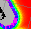
\includegraphics[width=0.75\textwidth]{images/costmap_2d_costgradient}
\caption{costmap\_2d sample \label{fig:costmap_2d_costgradient}}
\end{figure}

For obstacle mapping, the ROS navigation stack uses a software package called ``costmap\_2d" \todo{reference to costmap2d wiki page}. This package takes in sensor information about the environment, builds a 2D or 3D fixed-resolution occupancy grid by raytracing that sensor information and inflates obstacles to facilitate navigation based on user provided robot parameters. For a visualization of a small portion of a costmap built from actual sensor data, see \autoref{fig:costmap_2d_costgradient}. In \autoref{fig:costmap_2d_costgradient} black pixels are the actual sensed obstacles, gray pixels are marked as "lethal" cost and the rest are a gradient between high cost in violet and low cost in red. Lethal cells are obstacles that have been inflated according the robot's geometry - specifically these are any cells that if the control point (or origin/center) of the robot were to enter one of these cells it would be in collision with the actual sensed obstacle. Outside of this inflated radius (also known as configuration space \todo{reference to configuration space}), the cost gradient expresses a preference for the path planners to stay away from obstacles unless other factors force the robot near to the obstacle.

While this approach works in many environments, it has drawbacks when used for precision navigation. The most serious drawback is the fixed resolution of the grid when very fine resolution is required for some areas, but not others. For example, imagine navigating through a narrow doorway that opens to wide open areas on either side. In this situation, there is generally no good overall choice for the resolution of the grid. Choosing a resolution that is fine enough to ensure that the robot can always fit through the doorway leads to an unnecessarily large number of empty cells in the wide open areas, wasting both memory and computation time evaluating these cells; choosing a resolution that reduces the number of cells in the open areas may not guarantee that the doorway will always be sensed as traversable, as even a sensor reading along an edge of a cell will cause the entire cell to be marked as an obstacle. While prior knowledge about an environment allows one to choose a good resolution for that environment, that choice may not be optimal for a different environment; even if an ``adaptive" fixed resolution were used that was always optimal for representing a given environment, path planning performance, both how long it takes to find an optimal plan and the actual optimal plan generated, can be affected by changing the obstacle map resolution, which is undesirable for a navigation system that seeks to perform consistently in different environments.

Another issue with the implementation used by costmap\_2d is that, with a very fine grid cell resolution, obstacles can leave ``droppings" in the map. These ``droppings" occur when an obstacle such as a human moves across the sensor's field of view and is not completely cleared out of the map because the raytraced sensor beams do not intersect all of the cells that had already been marked as occupied. In order to resolve this problem, either a large enough grid cell resolution must be used to ensure that sensor beams will never fall to either side of an occupied cell (but, as discussed previously, large grid cell resolutions have other significant drawbacks) or an occupancy grid implementation that can clear cells even if a sensor beam does not raytrace through a particular cell must be used. For example, an occupancy grid implementation could slowly ``fade" obstacle cells so that obstacles that have not been observed for some time would automatically be cleared. Other possibilities include explicitly modeling the probability of each cell given all of the previous sensor measurements, such as the occupancy grid mappying techniques introduced in \autocite{Moravec_1985_1840}. The proposed mapping solution used in this thesis is detailed in \todo{reference section where I talk about octocostmap and costmap3d}.

\subsection{Local Planning}\label{subsec:base_local_planner}

For local planning, the ROS navigation stack uses a software package called ``base\_local\_planner" \todo{reference to baseLocalPlanner wiki page}. This package uses the occupancy grid built by the package described in \autoref{subsec:costmap_2d} to generate steering commands (translational velocity and rotational velocity) such that the robot follows a given path through the environment without collisions. To do this, base\_local\_planner, as configured for HARLIE, uses an algorithm called Trajectory Rollout \autocite{Gerkey_Konolige_2008}. The algorithm can be described as a sequence of four steps that are repeated until the robot reaches the end of the path. The steps are as follows:
\begin{enumerate}
\item Sample the robot's control space, generate translational (forward) velocity and rotational velocity pairs. These pairs are the possible commands that could be sent to the robot, given it's current state and dynamics constraints (e.g. acceleration).
\item Forward simulate each of those control pairs for some short, fixed amount of time to determine what would happen if the robot were given that control pair. One forward simulated control pair creates one possible trajectory.
\item Score each trajectory using a cost function \eqref{base_local_planner_cost_func} to determine the ``goodness" of a trajectory. Discard any trajectories that result in collisions.
\item Pick the trajectory that scores the best (this could be lowest or highest score depending on cost function) and send the control pair that generated that trajectory to the robot.
\end{enumerate}

The scoring function used by the Trajectory Rollout implementation in base\_local\_planner is as follows:
\begin{equation}
	k_{path} \cdot pathDist + k_{goal} \cdot goalDist + k_{obs} \cdot obs \label{base_local_planner_cost_func}
\end{equation}
In \eqref{base_local_planner_cost_func}, the three $k$ terms are weights that control how much each of the individual cost components influence the overall score. The three cost components are $pathDist$, $goalDist$ and $obs$. $pathDist$ is the distance between the endpoint of the trajectory and the closest point on the path. $goalDist$ is the distance between the endpoint of the trajetory and the end of the given path. $obs$ is the maximum cost for any point along the trajectory as returned by the occupancy grid. A visualization of the cost function components and sum for one cycle is in \autoref{fig:base_local_planner_cost_visualization}.

\begin{figure}
\centering
\subfloat[Obstacle Cost]{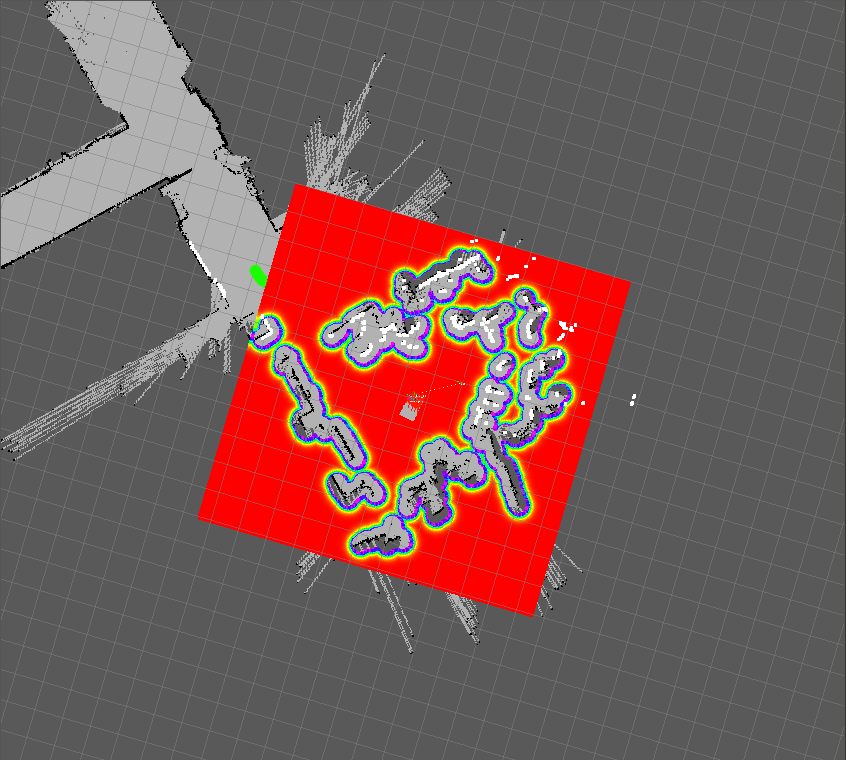
\includegraphics[width=0.5\textwidth]{images/obstacle_cost}\label{fig:obstacle_cost}}
\hfill
\subfloat[Goal Cost]{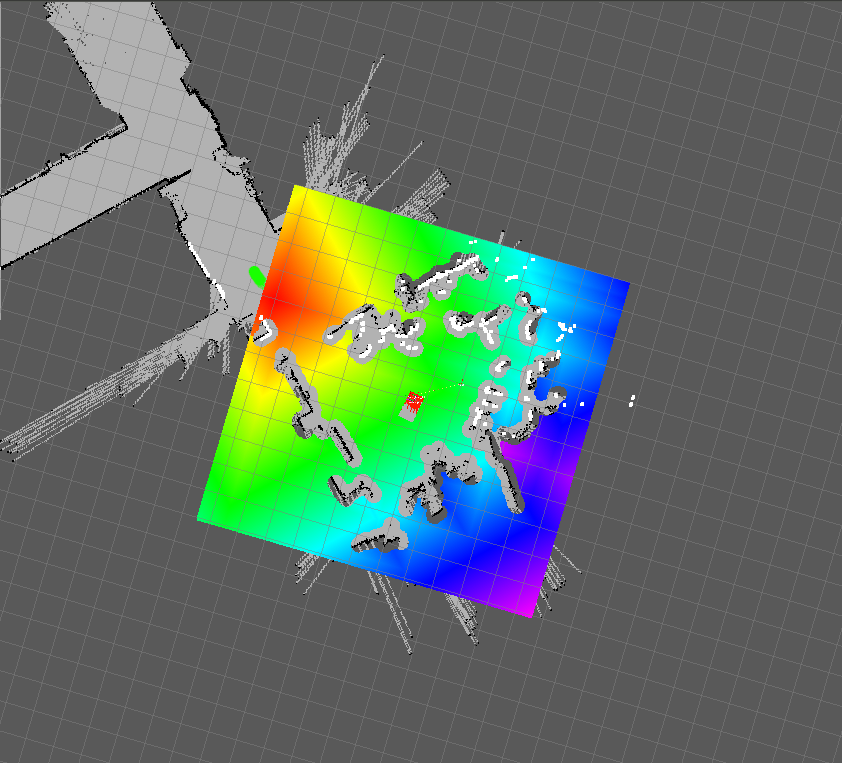
\includegraphics[width=0.5\textwidth]{images/goal_cost}\label{fig:goal_cost}}
\\
\subfloat[Path Cost]{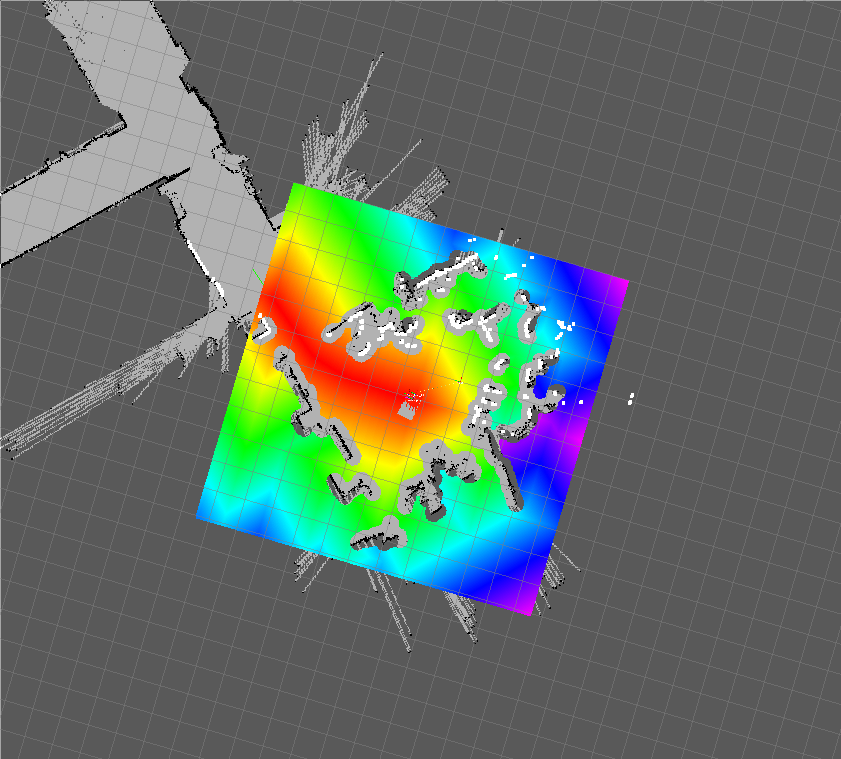
\includegraphics[width=0.5\textwidth]{images/path_cost}\label{fig:path_cost}}
\hfill
\subfloat[Total Cost]{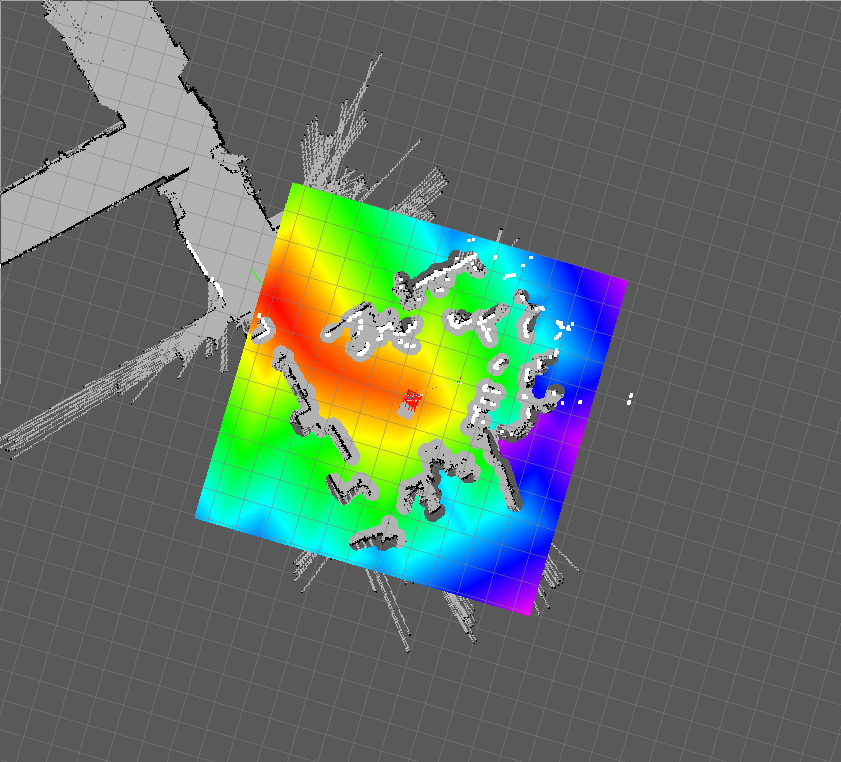
\includegraphics[width=0.5\textwidth]{images/total_cost}\label{fig:total_cost}}
\caption[Sample Trajectory Rollout Cost Visualization]{Sample Trajectory Rollout Cost Visualization. The robot is in the center of the cost field. The end of the commanded path is visible as a green line to the upper left of the cost field. Red is low cost. Violet is high cost.}
\label{fig:base_local_planner_cost_visualization}
\end{figure}

There are a number of issues that arise from using this type of method when attempting to do precision navigation of a differential drive robot. One such issue is the simplistic generation of trajectories. In base\_local\_planner, trajectories are generated using a fixed number of samples between the minimum and maximum translational velocities that could be commanded to the robot, given the current translational velocity and acceleration and deceleration limits, and similarly sampling from the possible rotational velocity space. The trajectories are then generated by forward simulation of the cartesian product of these two sets of velocities (see \todo{insert figure of sample trajectories that are evaluated by BaseLocalPlanner} for an example set of trajectories). The problem with this method of generating trajectories is two-fold. First, the number of samples must remain relatively small compared to the overall possible controls space in order to forward simulate and score all trajectories quickly (commands should be sent to the robot at 20Hz, so a control pair must be chosen at least every 20Hz), so a trajectory that may actually be better in the long term may not be evaluated if it was not one of the samples. Second, because one control pair is chosen per forward simulation, only short, constant curvature trajectories are evaluated. While these two problems do not generally affect navigation in environments where the circumscribed radius of the robot can pass through the smallest gap it must navigate (i.e. for a rectangular robot it could fit through sideways), they quickly lead to undesirable behavior in situations such as robotic wheelchairs passing through ADA compliant doorways or any other case where the robot must precisely follow the given path. In such situations, these simplistic trajectories do not ensure that the robot will be able to pass through the doorway smoothly --- for example, base\_local\_planner often needs to back up and re-align the robot once it gets close to the doorway because the trajectories that were scored and chosen did not lead to the robot being lined up such that it could pass straight through the doorway. 

Aother issue with using Trajectory Rollout for precision navigation is the simplistic scoring function used. The specific cost function used by base\_local\_planner \eqref{base_local_planner_cost_func} has only three components, which should cause the planner to choose trajectories that remain far away from obstacles, end near the goal and remain near the path. In practice, these few components are insufficient for precision navigation. For example, it is entirely possible for the planner to choose a trajectory that avoids obstacles and gets close to the goal, but doesn't follow the given path very closely even though it has the best score. This comes about because the distance to the path is only calculated from the endpoint of the trajectory and therefore is not some measure of overall fit of the entire trajectory to the given path. Another issue with this scoring function is its inablilty to handle spin-in-place actions. For a differential drive robot, these are an important ability when attempting to navigate in constrained environments (in the example above, a spin-in-place could be used for realigning to the doorway) but, because this scoring function prefers trajectories that move towards the goal and/or path, spin-in-place trajectories are rarely chosen, even if a spin-in-place would actually be a more optimal choice for getting to the goal sooner. Spin-in-place actions are not as important for a holonomic robot, as it can often just strafe instead of or while realigning; the preference of the cost function towards trajectories that move the robot closer to the goal and/or path still works when strafing, since strafing is more than just a change in heading.

\subsection{Global Planning}\label{subsec:navfn}

For global planning, the ROS navigation stack uses a package called ``navfn" \todo{insert ref to navfn wiki page}. This package uses the occupancy grid built by the package described in \autoref{subsec:costmap_2d} to generate the minimum cost plan between the robot's starting position and a given goal location. To do this, ``navfn" uses Dijkstra's shortest path algortihm as described in \autocite{Lav06}, assuming the robot has a circular projection onto the costmap. While this method does generate optimal paths that avoid obstacles, it has some shortcomings when used for precision navigation on robots such as HARLIE.

The most serious of these shortcomings is the circular robot assumption. For a robot such as HARLIE, which has an approximately 3:2 length:width footprint for the base, there are two choices for the radius of this circular robot approximation: the inscribed radius or the circumbscribed radius. If the inscribed radius is chosen, ``navfn" is planning paths between obstacles that the robot can actually pass through, but the planner may generate paths that cause the back end to hit obstacles. An example of this situation is when planning an L-shape through a narrow doorway --- after the path passes through the midpoint of the doorway, it will turn too early and, if the path is followed precisely, cause the back of the robot to swing into the door as it turns. On the other hand, if the circumscribed radius is chosen ``navfn" will not be able to plan a path through all environments that the robot can actually navigate because the planner will, essentially, be trying to fit the robot through sideways. Any global planner used for precision navigation must use the actual footprint of the robot so that it plans paths in any environment the robot can safely navigate while not underestimating the size of the robot and generating paths that may lead to collisions.


Another issue with ``navfn" as the global planner in a precision navigation application is that it is not a dynamic planning algorithm. Dijkstra's algorithm (and other static path planning algortihms such as A*) must replan from scratch if the environment changes during execution; to achieve precise navigation in arbitrary environments, any planner used must handle dynamic obstacles such as people or other robots. Dynamic planning algorithms such as Field D* \autocite{FieldDStar} or ADA* \autocites{ADAStar}{DBLP:journals/ai/LikhachevFGST08} are designed to adjust the planned path to account for dynamic obstacles with a minimum of recomputation. Because of this, the plan can continuously be refined or a larger, more flexible state space used, leading to smoother, better overall plans; Dijkstra's would need a relatively small state space in order to recompute the entire path quickly to account for dyanmic obstacles.

\begin{comment}
This will detail problems in ROS's Navigation stack when we last looked at it (and perhaps a discussion of how it has changed in the interim)

Outline:
	Mapping
		SimpleCostmap
		Fixed Grid size - needs changed for different environments and may affect trajectory scoring
		No option for temporal clearing of the map to reduce "leftovers" at small resolutions
	Local planning
		Scoring of trajectories
		Trajectories come from a fixed list of velocities and omegas (cross-product)
		simplistic cost function
		holonomic vs diff-drive
		scoring spin-in-place
	global planning
		dijkstra's planning
		replan only as a last resort
		may generate crappy plan since uses a circular robot with either inscribed or circumscribed radius
	localization
		defaults require tweaking for both map building and amcl
		amcl needs tuned to prevent "pops"
		
\end{comment}
